%!TEX root = ../report.tex
\documentclass[../report.tex]{subfiles}

\begin{document}
    \section*{APPENDIX}
    \label{sec:appendix}
    This appendix provides supplementary information and additional results that complement the main text of the report.

    \subsection*{A.1 List of Abbreviations}
    \label{subsec:abbreviations}
    Table~\ref{tab:abbreviations} lists all abbreviations used throughout this report for quick reference.
    \begin{table}[ht]
        \caption{List of Abbreviations used throughout the report}
        \label{tab:abbreviations}
        \centering
        \begin{tabular}{{M{0.45\linewidth} M{0.45\linewidth}}}
            \hline
            \cellcolor{gray!10!white} Abbreviation & \cellcolor{gray!10!white} Full Form  \\\hline
            AI & Artificial Intelligence \\\hline
            ASR & Automatic Speech Recognition \\\hline
            AtMan & Attention Manipulation \\\hline
            CAM & Class Activation Mapping \\\hline
            DNN & Deep Neural Network \\\hline
            LIME & Local Interpretable Model-agnostic Explanations \\\hline
            NLP & Natural Language Processing \\\hline
            NMF & Non-negative Matrix Factorization \\\hline
            POC & Proof of Concept \\\hline
            SHAP & SHapley Additive exPlanations \\\hline
            STFT & Short-Time Fourier Transform \\\hline
            ViT & Vision Transformer \\\hline
            XAI & Explainable Artificial Intelligence \\\hline
        \end{tabular}
    \end{table}

    \subsection*{A.2 Implementation Details}
    \label{subsec:implementation}
    The complete implementation of this project, including the AtMan framework and all experiments, is available as open-source software at \url{https://github.com/arunimaCh29/AtMan-Whisper}. The repository contains detailed documentation and instructions for reproducing our results.

    \subsection*{A.3 Additional Visualization Examples}
    \label{subsec:additional_viz}
    This section presents additional examples of our visualization methodology, complementing the results discussed in Section~\ref{sec:evaluation}. For each example, we show:
    \begin{itemize}
        \item The input audio's log-mel spectrogram
        \item The sentence-level influence map showing overall attention patterns
        \item Token-level influence maps highlighting word-specific patterns
    \end{itemize}
    These visualizations further demonstrate the effectiveness of our approach in explaining the Whisper model's behavior across various input scenarios.

    \subsubsection*{A.3.1 Short Utterance Analysis}
    Figure~\ref{fig:viz_set1} shows the analysis of a short utterance, demonstrating how our method handles concise speech segments.
    \begin{figure*}[p]
        \centering
        \begin{minipage}{0.95\textwidth}
        \raggedright
        \textbf{Transcription 1:} \textit{Well now Ennis I declare you have a head and so has my stick}
        \end{minipage}
        
        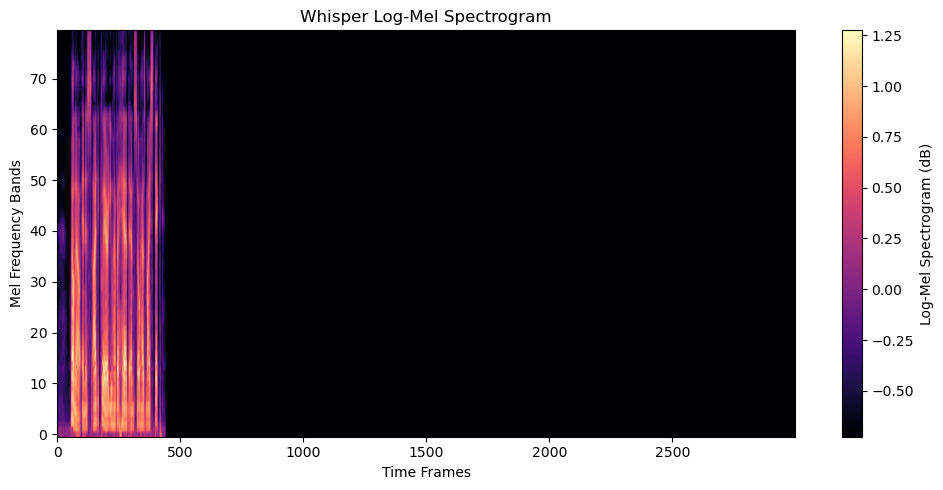
\includegraphics[width=0.5\textwidth]{figures/mel1.png}
        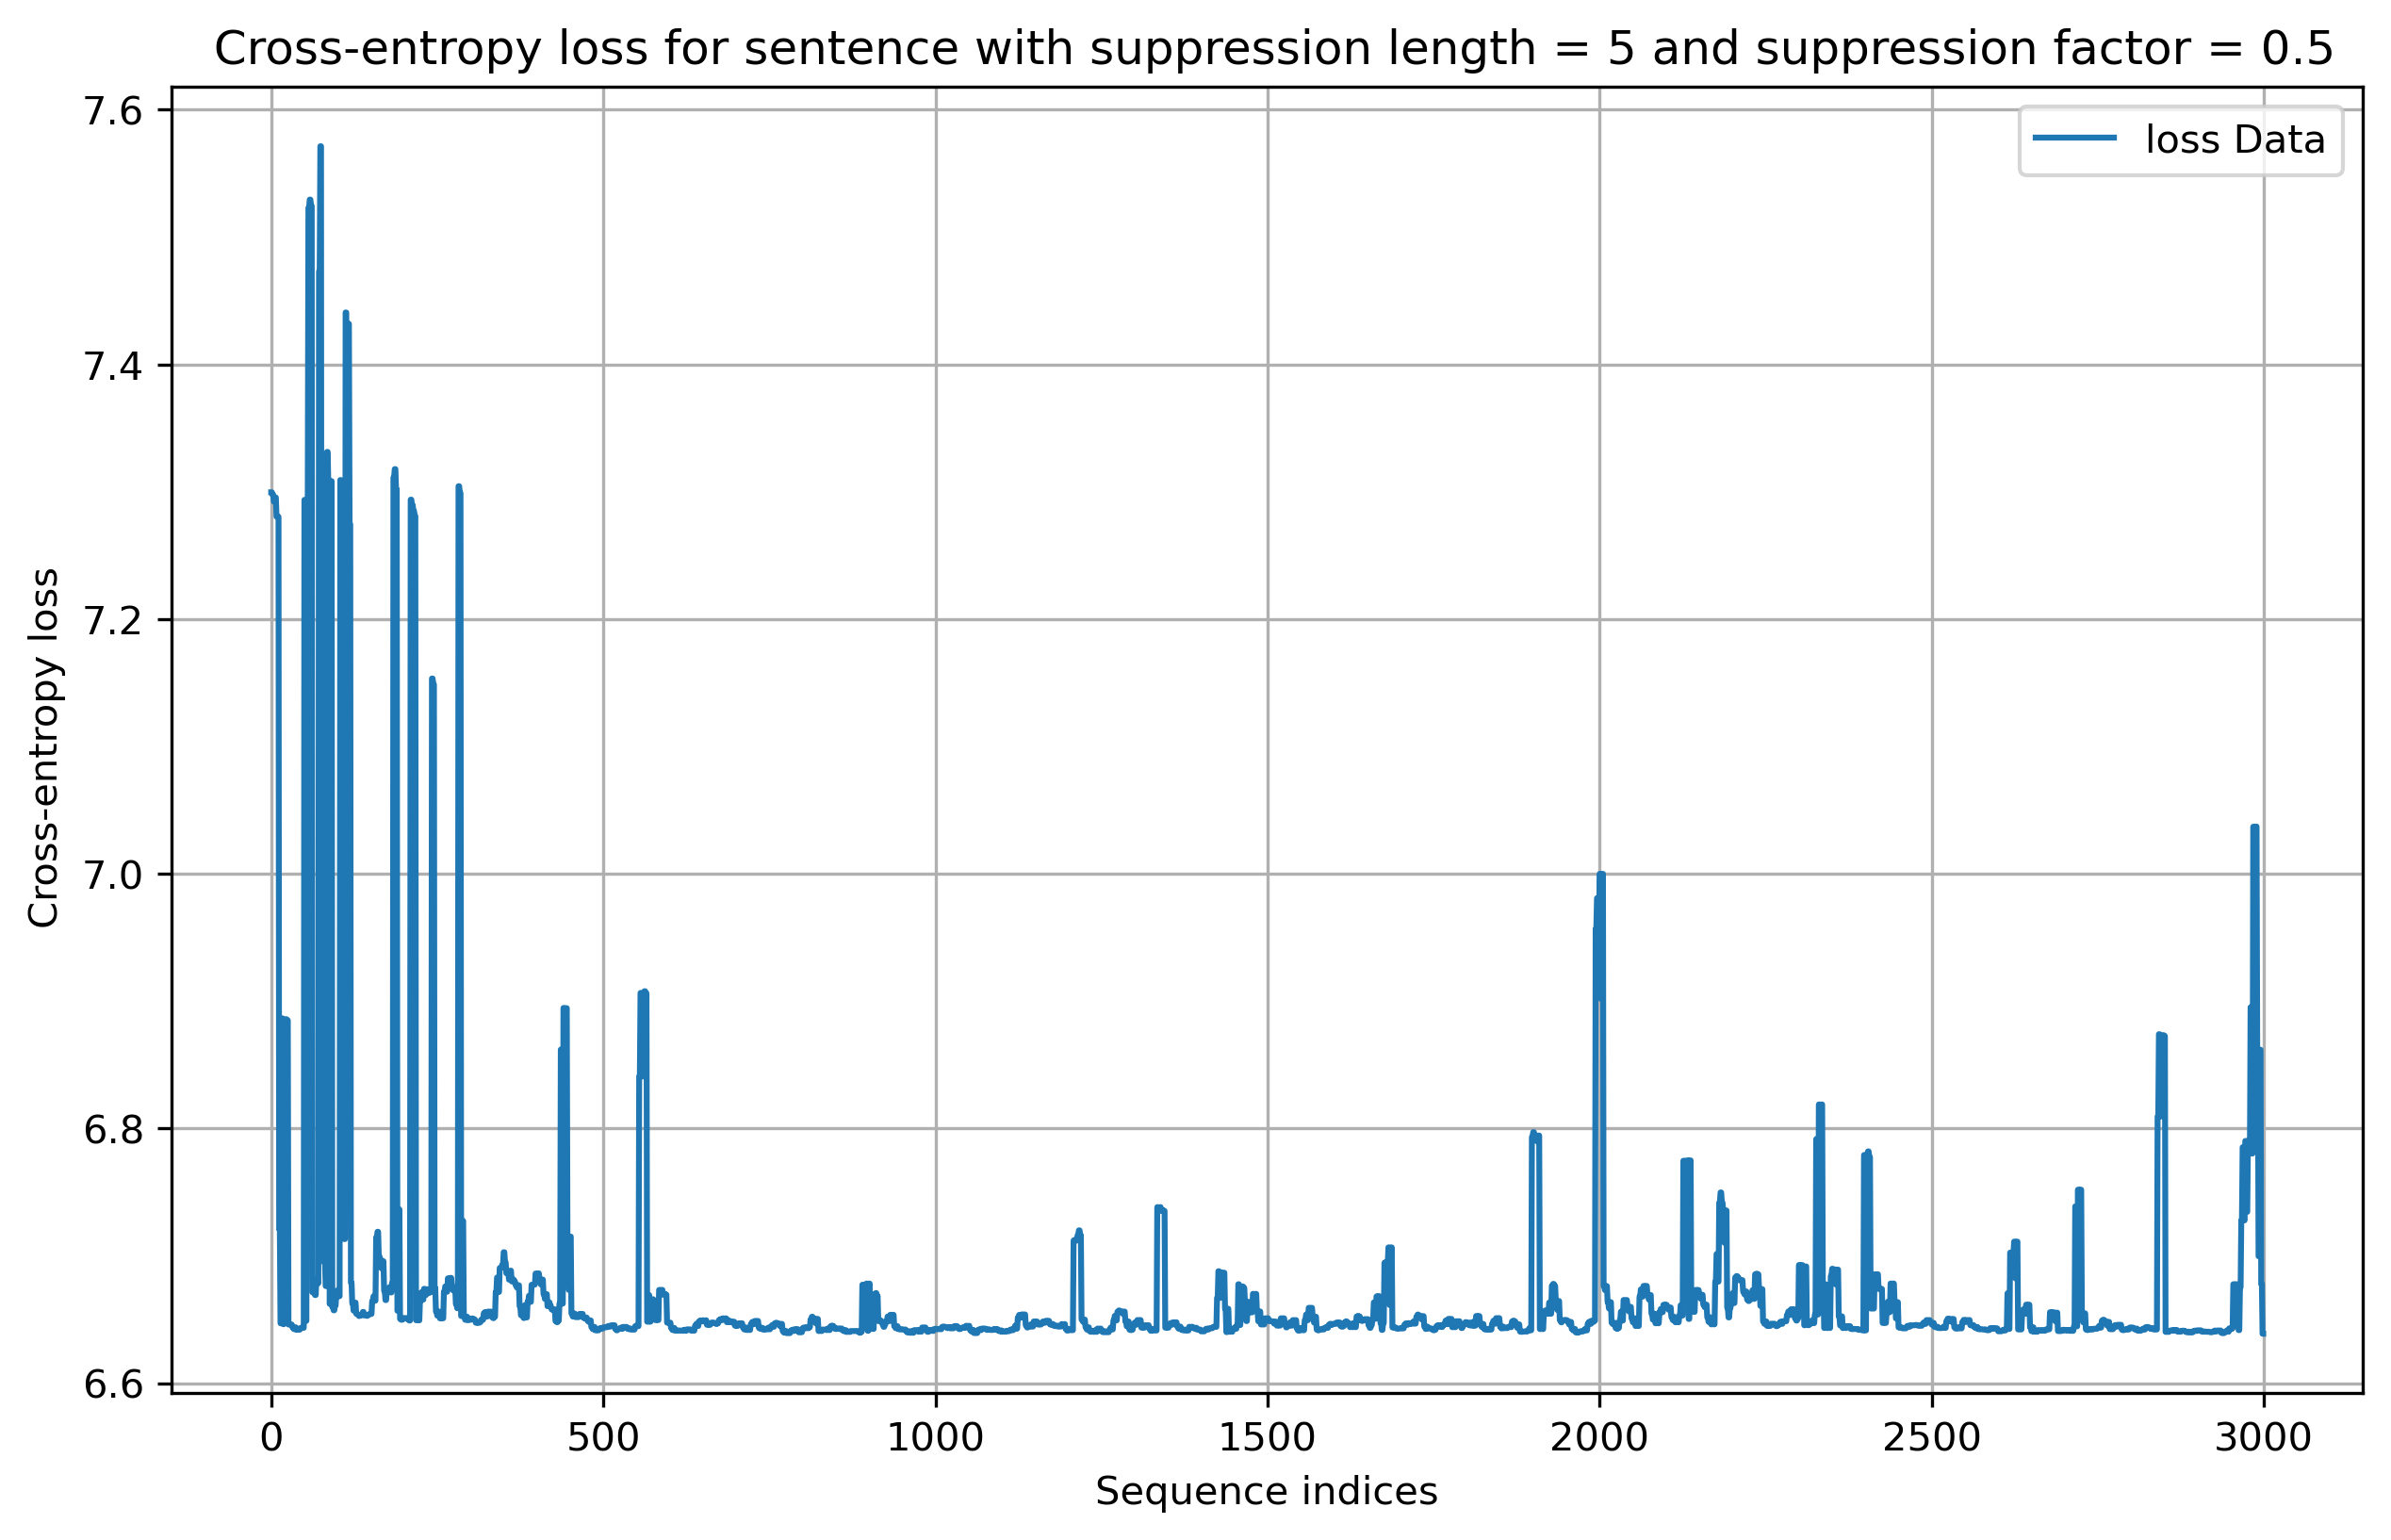
\includegraphics[width=0.5\textwidth]{figures/loss_diff_sentence_1_sentence.png}
        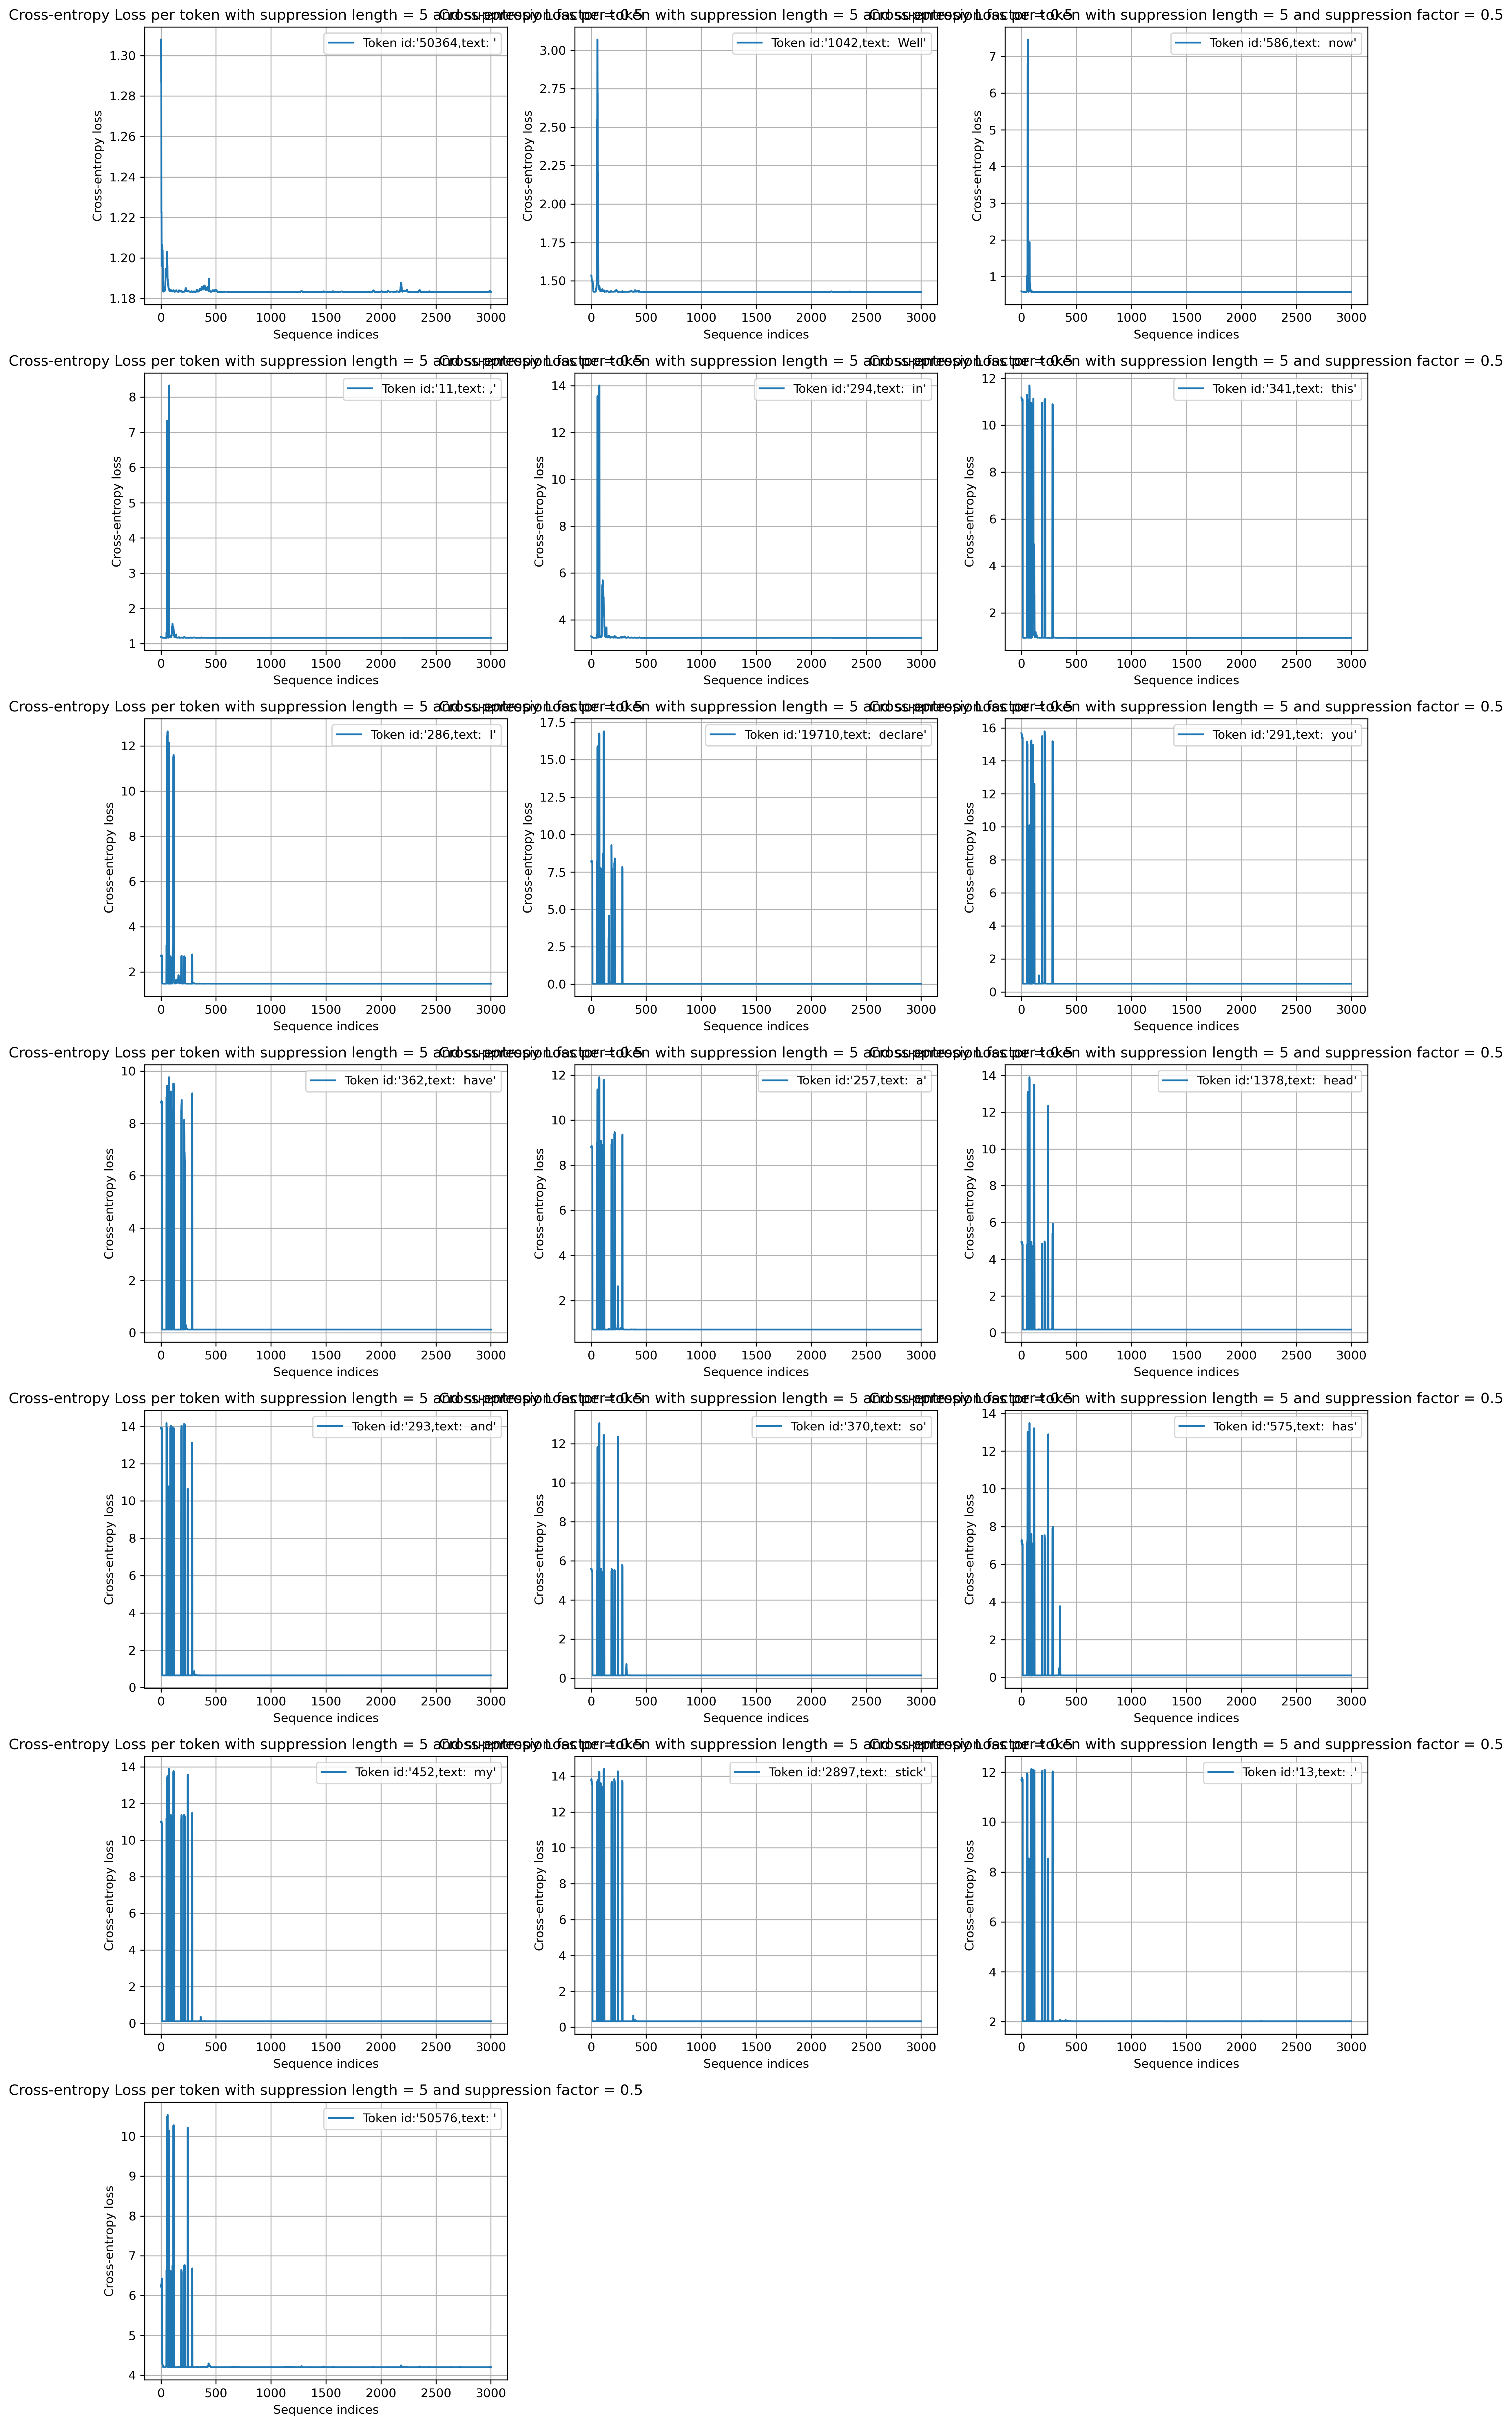
\includegraphics[width=\textwidth,height=0.45\textheight]{figures/loss_diff_sentence_1_word.png}
        \caption{Analysis of a short utterance showing (top) log-mel spectrogram, (middle) sentence-level influence map highlighting overall attention patterns, and (bottom) token-level influence maps revealing word-specific attention distributions.}
        \label{fig:viz_set1}
    \end{figure*}

    \subsubsection*{A.3.2 Complex Sentence Structure}
    Figures~\ref{fig:viz_set2} and~\ref{fig:viz_set3} demonstrate our method's capability in handling complex sentence structures with multiple clauses.
    \begin{figure*}[p]
        \centering
        \begin{minipage}{0.95\textwidth}
        \raggedright
        \textbf{Transcription 2:} \textit{On Saturday mornings when the sodality met in the chapel to recite the little office his place was a cushioned kneeling desk at the right of the altar from which he led his wing of boys through the responses}
        \end{minipage}
        
        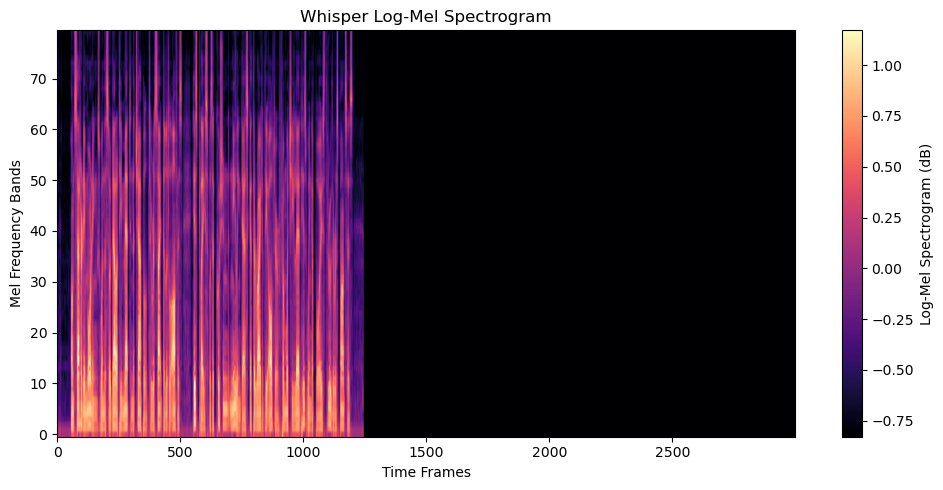
\includegraphics[width=0.5\textwidth]{figures/mel2.png}
        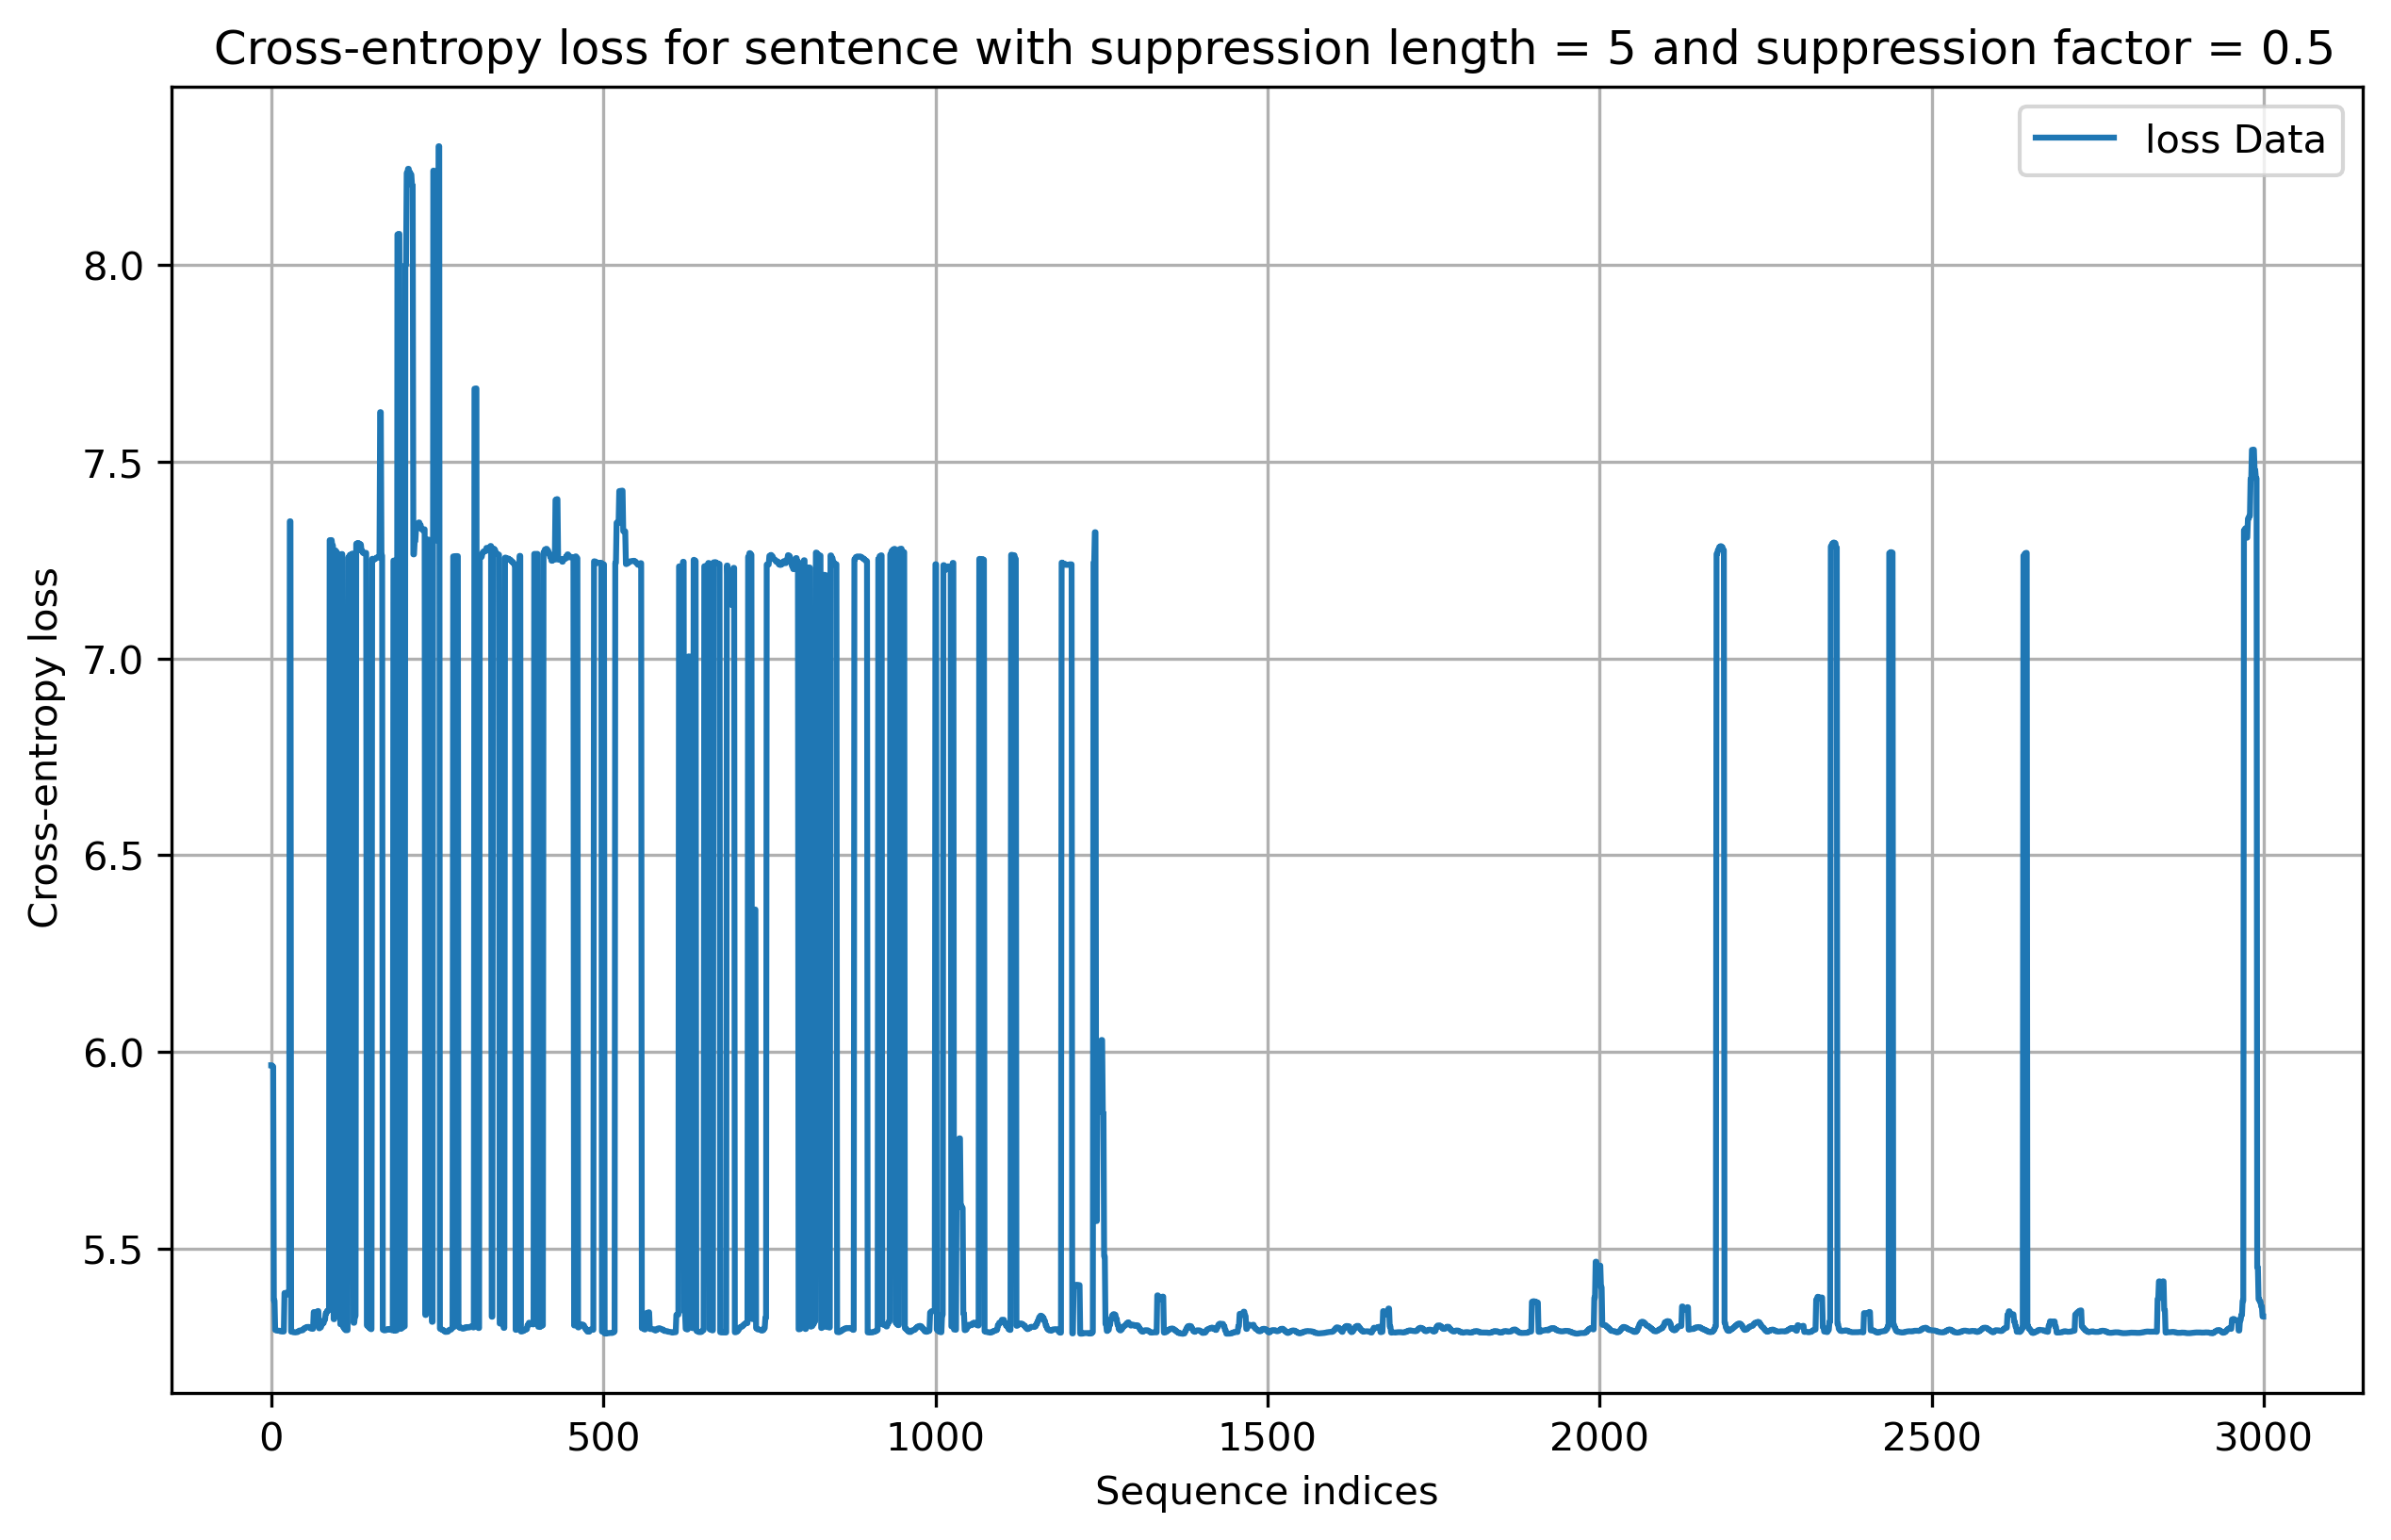
\includegraphics[width=0.5\textwidth]{figures/loss_diff_sentence_2_sentence.png}
        % \caption{Visualization set 2: (top) Log Mel spectrogram, (middle) sentence-level influence map}
        % \newpage
        \includegraphics[width=0.7\textwidth,height=0.5\textheight]{figures/loss_diff_sentence_2_word.png}
        \caption{Visualization set 2 (continued): token-level influence maps}
        \label{fig:viz_set2}
    \end{figure*}

    \begin{figure*}[p]
        \centering
        \begin{minipage}{0.95\textwidth}
        \raggedright
        \textbf{Transcription 3:} \textit{Her eyes seemed to regard him with mild pity her holiness a strange light glowing faintly upon her frail flesh did not humiliate the sinner who approached her}
        \end{minipage}
        
        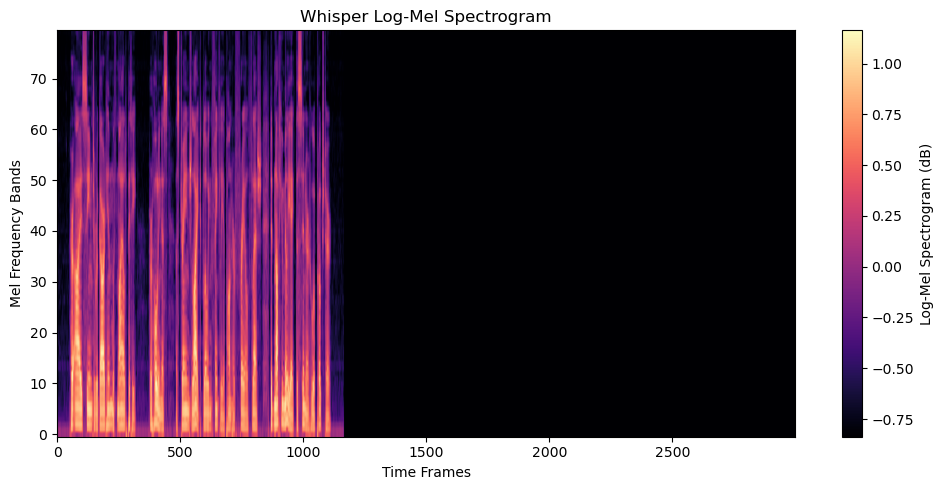
\includegraphics[width=0.5\textwidth]{figures/mel3.png}
        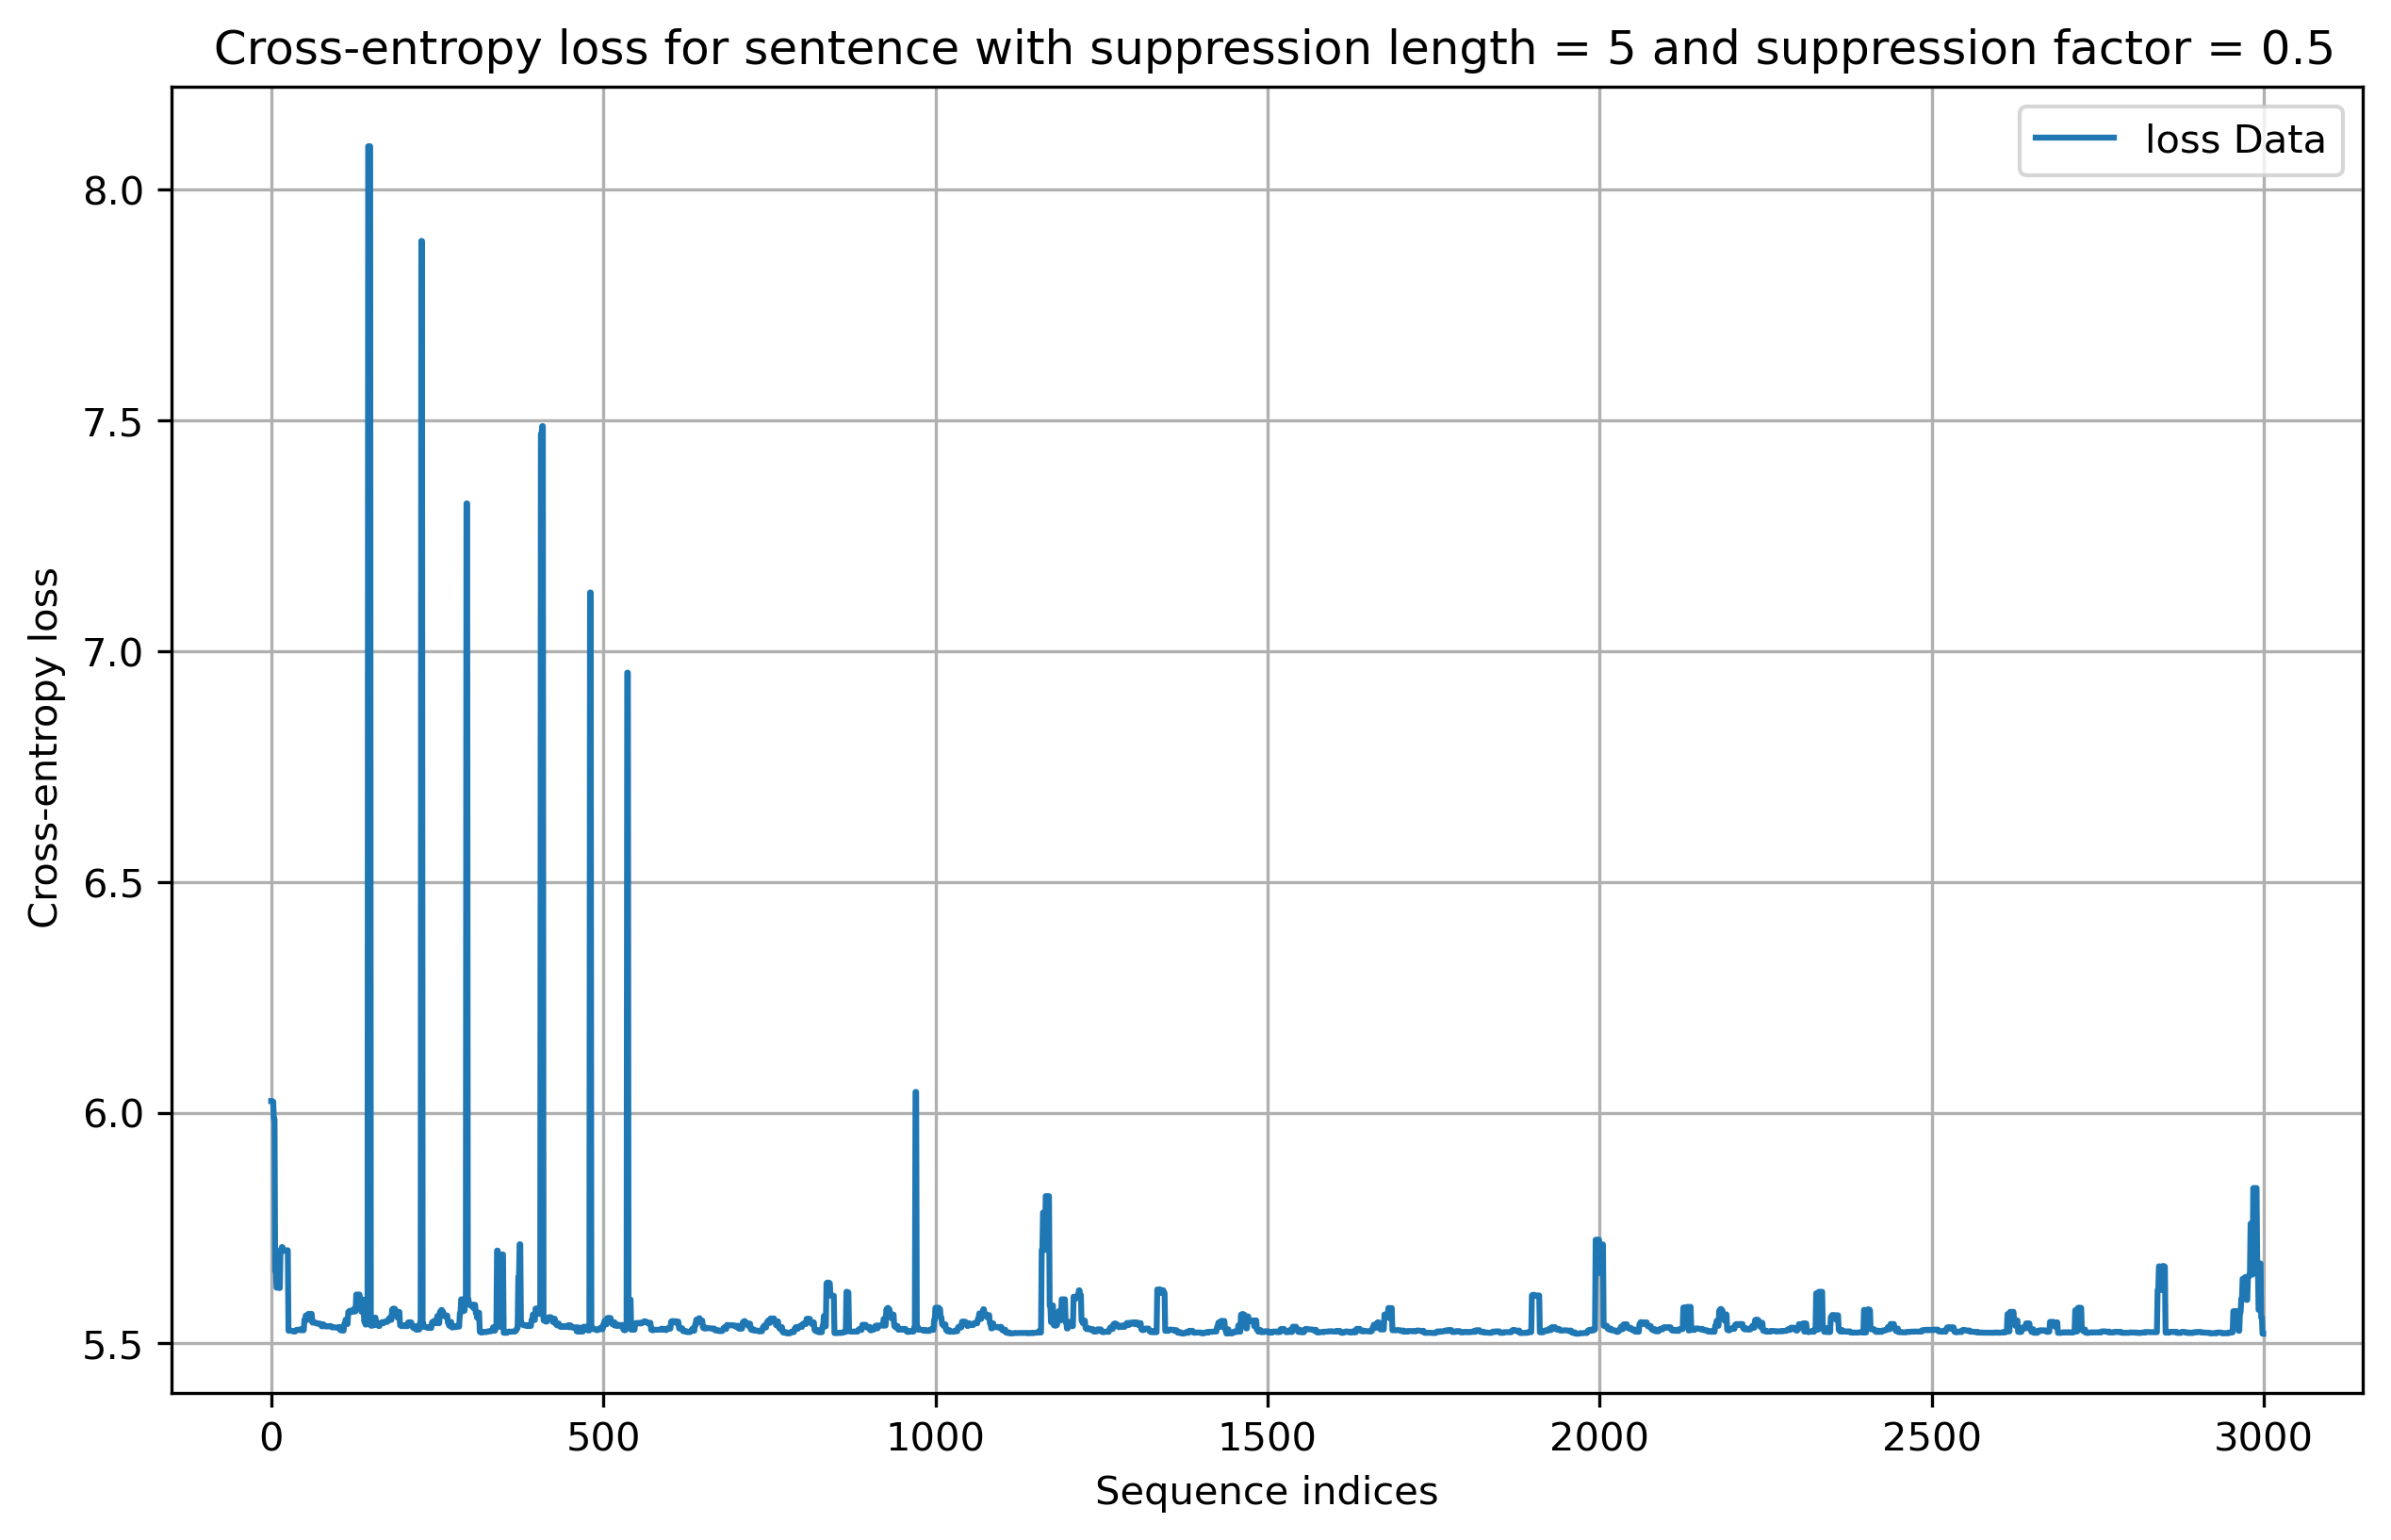
\includegraphics[width=0.5\textwidth]{figures/loss_diff_sentence_3_sentence.png}
        % \caption{Visualization set 3: (top) Log Mel spectrogram, (middle) sentence-level influence map}
        % \newpage
        \includegraphics[width=0.7\textwidth,height=0.5\textheight]{figures/loss_diff_sentence_3_word.png}
        \caption{Visualization set 3 (continued): token-level influence maps}
        \label{fig:viz_set3}
    \end{figure*}

    \begin{figure*}[p]
        \centering
        \begin{minipage}{0.95\textwidth}
        \raggedright
        \textbf{Transcription 4:} \textit{If ever he was impelled to cast sin from him and to repent the impulse that moved him was the wish to be her knight}
        \end{minipage}
        
        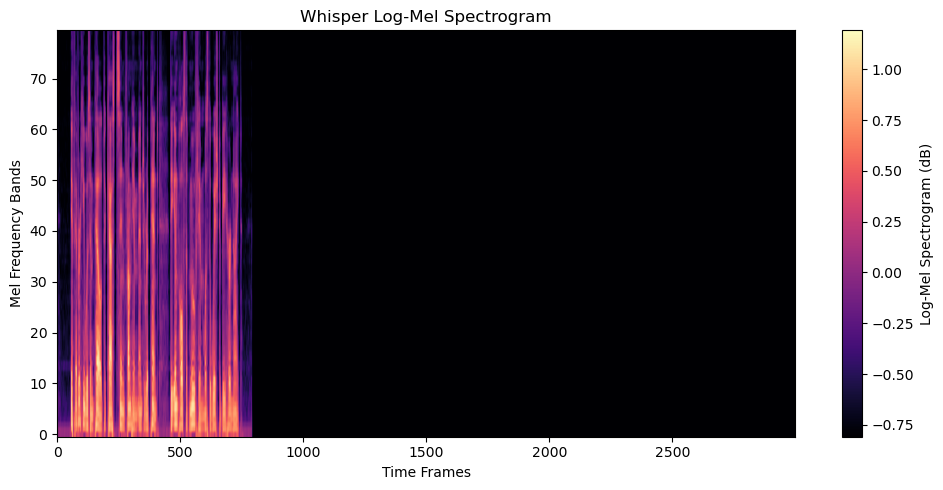
\includegraphics[width=0.5\textwidth]{figures/mel4.png}
        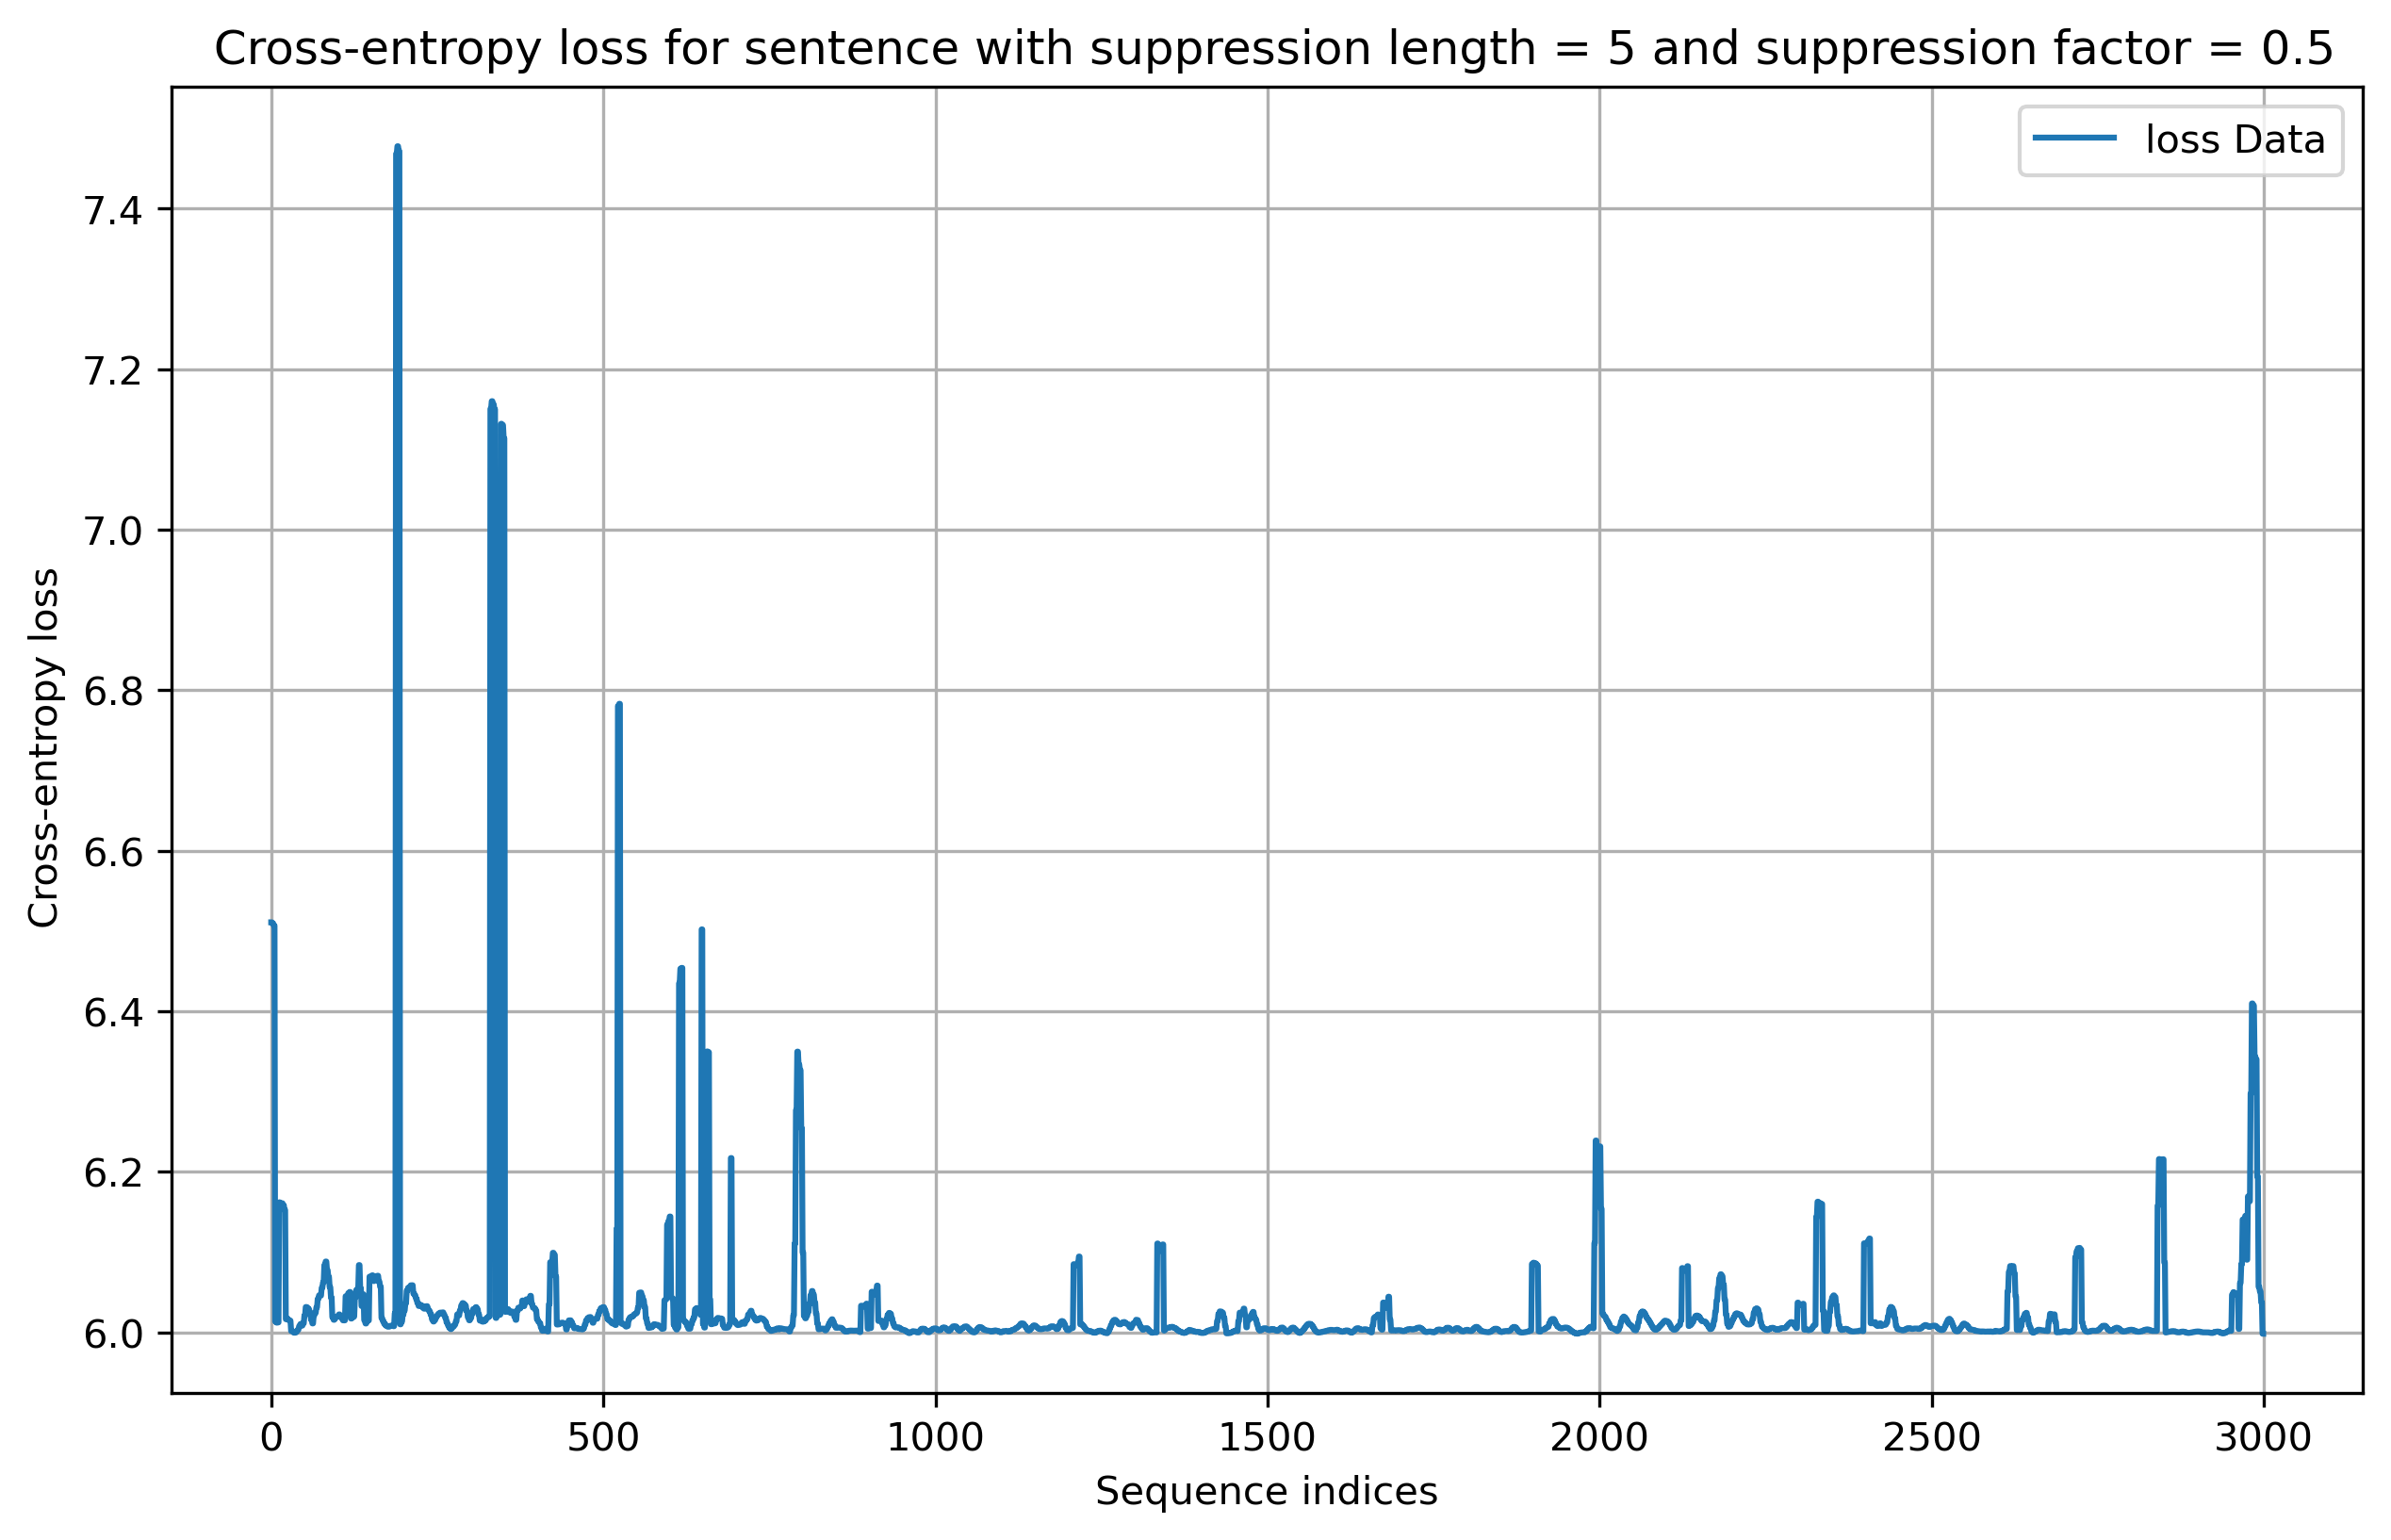
\includegraphics[width=0.5\textwidth]{figures/loss_diff_sentence_4_sentence.png}
        \includegraphics[width=0.7\textwidth,height=0.5\textheight]{figures/loss_diff_sentence_4_word.png}
        \caption{Visualization set 4: (top) Log Mel spectrogram, (middle) sentence-level influence map}
        \label{fig:viz_set4}
    \end{figure*}

    \begin{figure*}[p]
        \centering
        \begin{minipage}{0.95\textwidth}
        \raggedright
        \textbf{Transcription 5:} \textit{He tried to think how it could be}
        \end{minipage}
        
        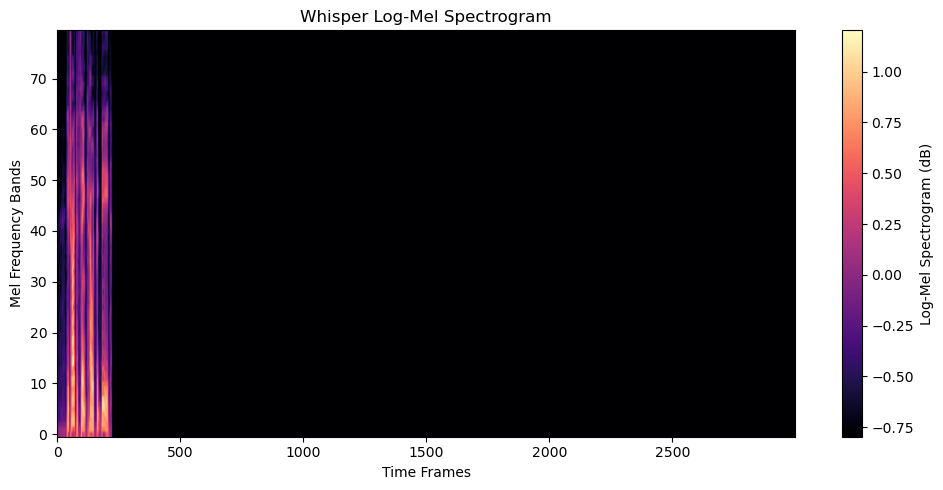
\includegraphics[width=0.5\textwidth]{figures/mel5.png}
        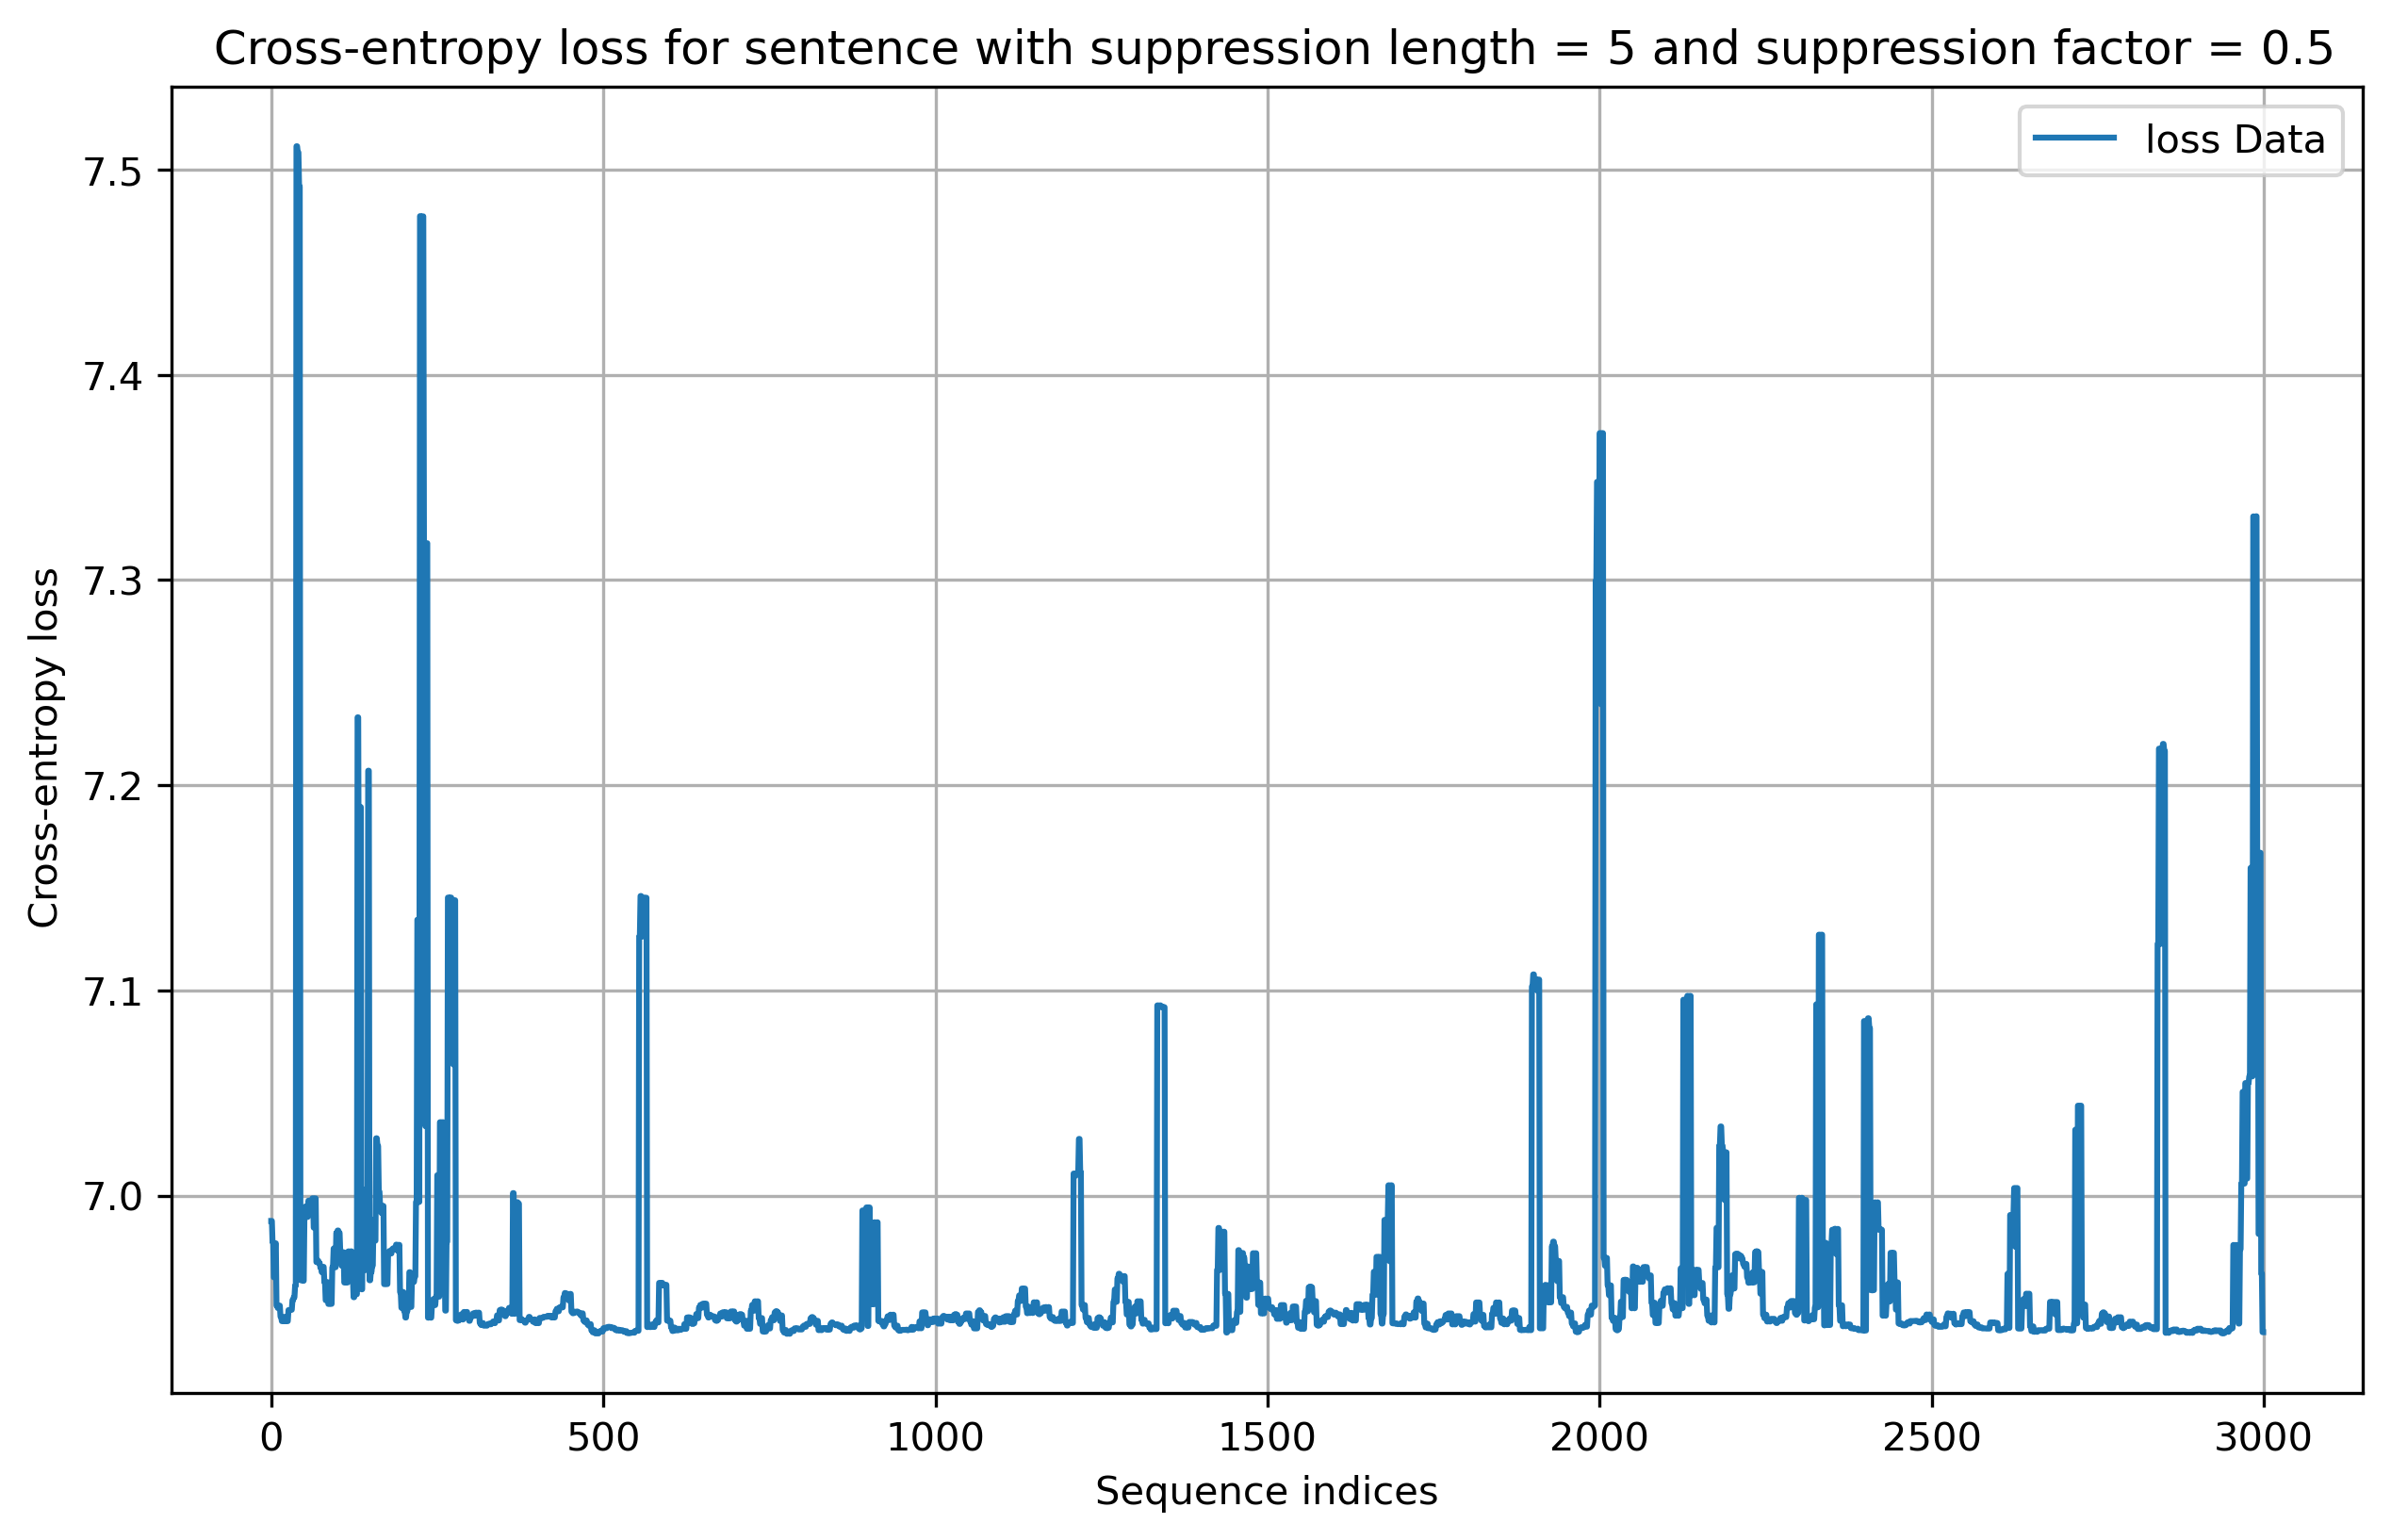
\includegraphics[width=0.5\textwidth]{figures/loss_diff_sentence_5_sentence.png}
        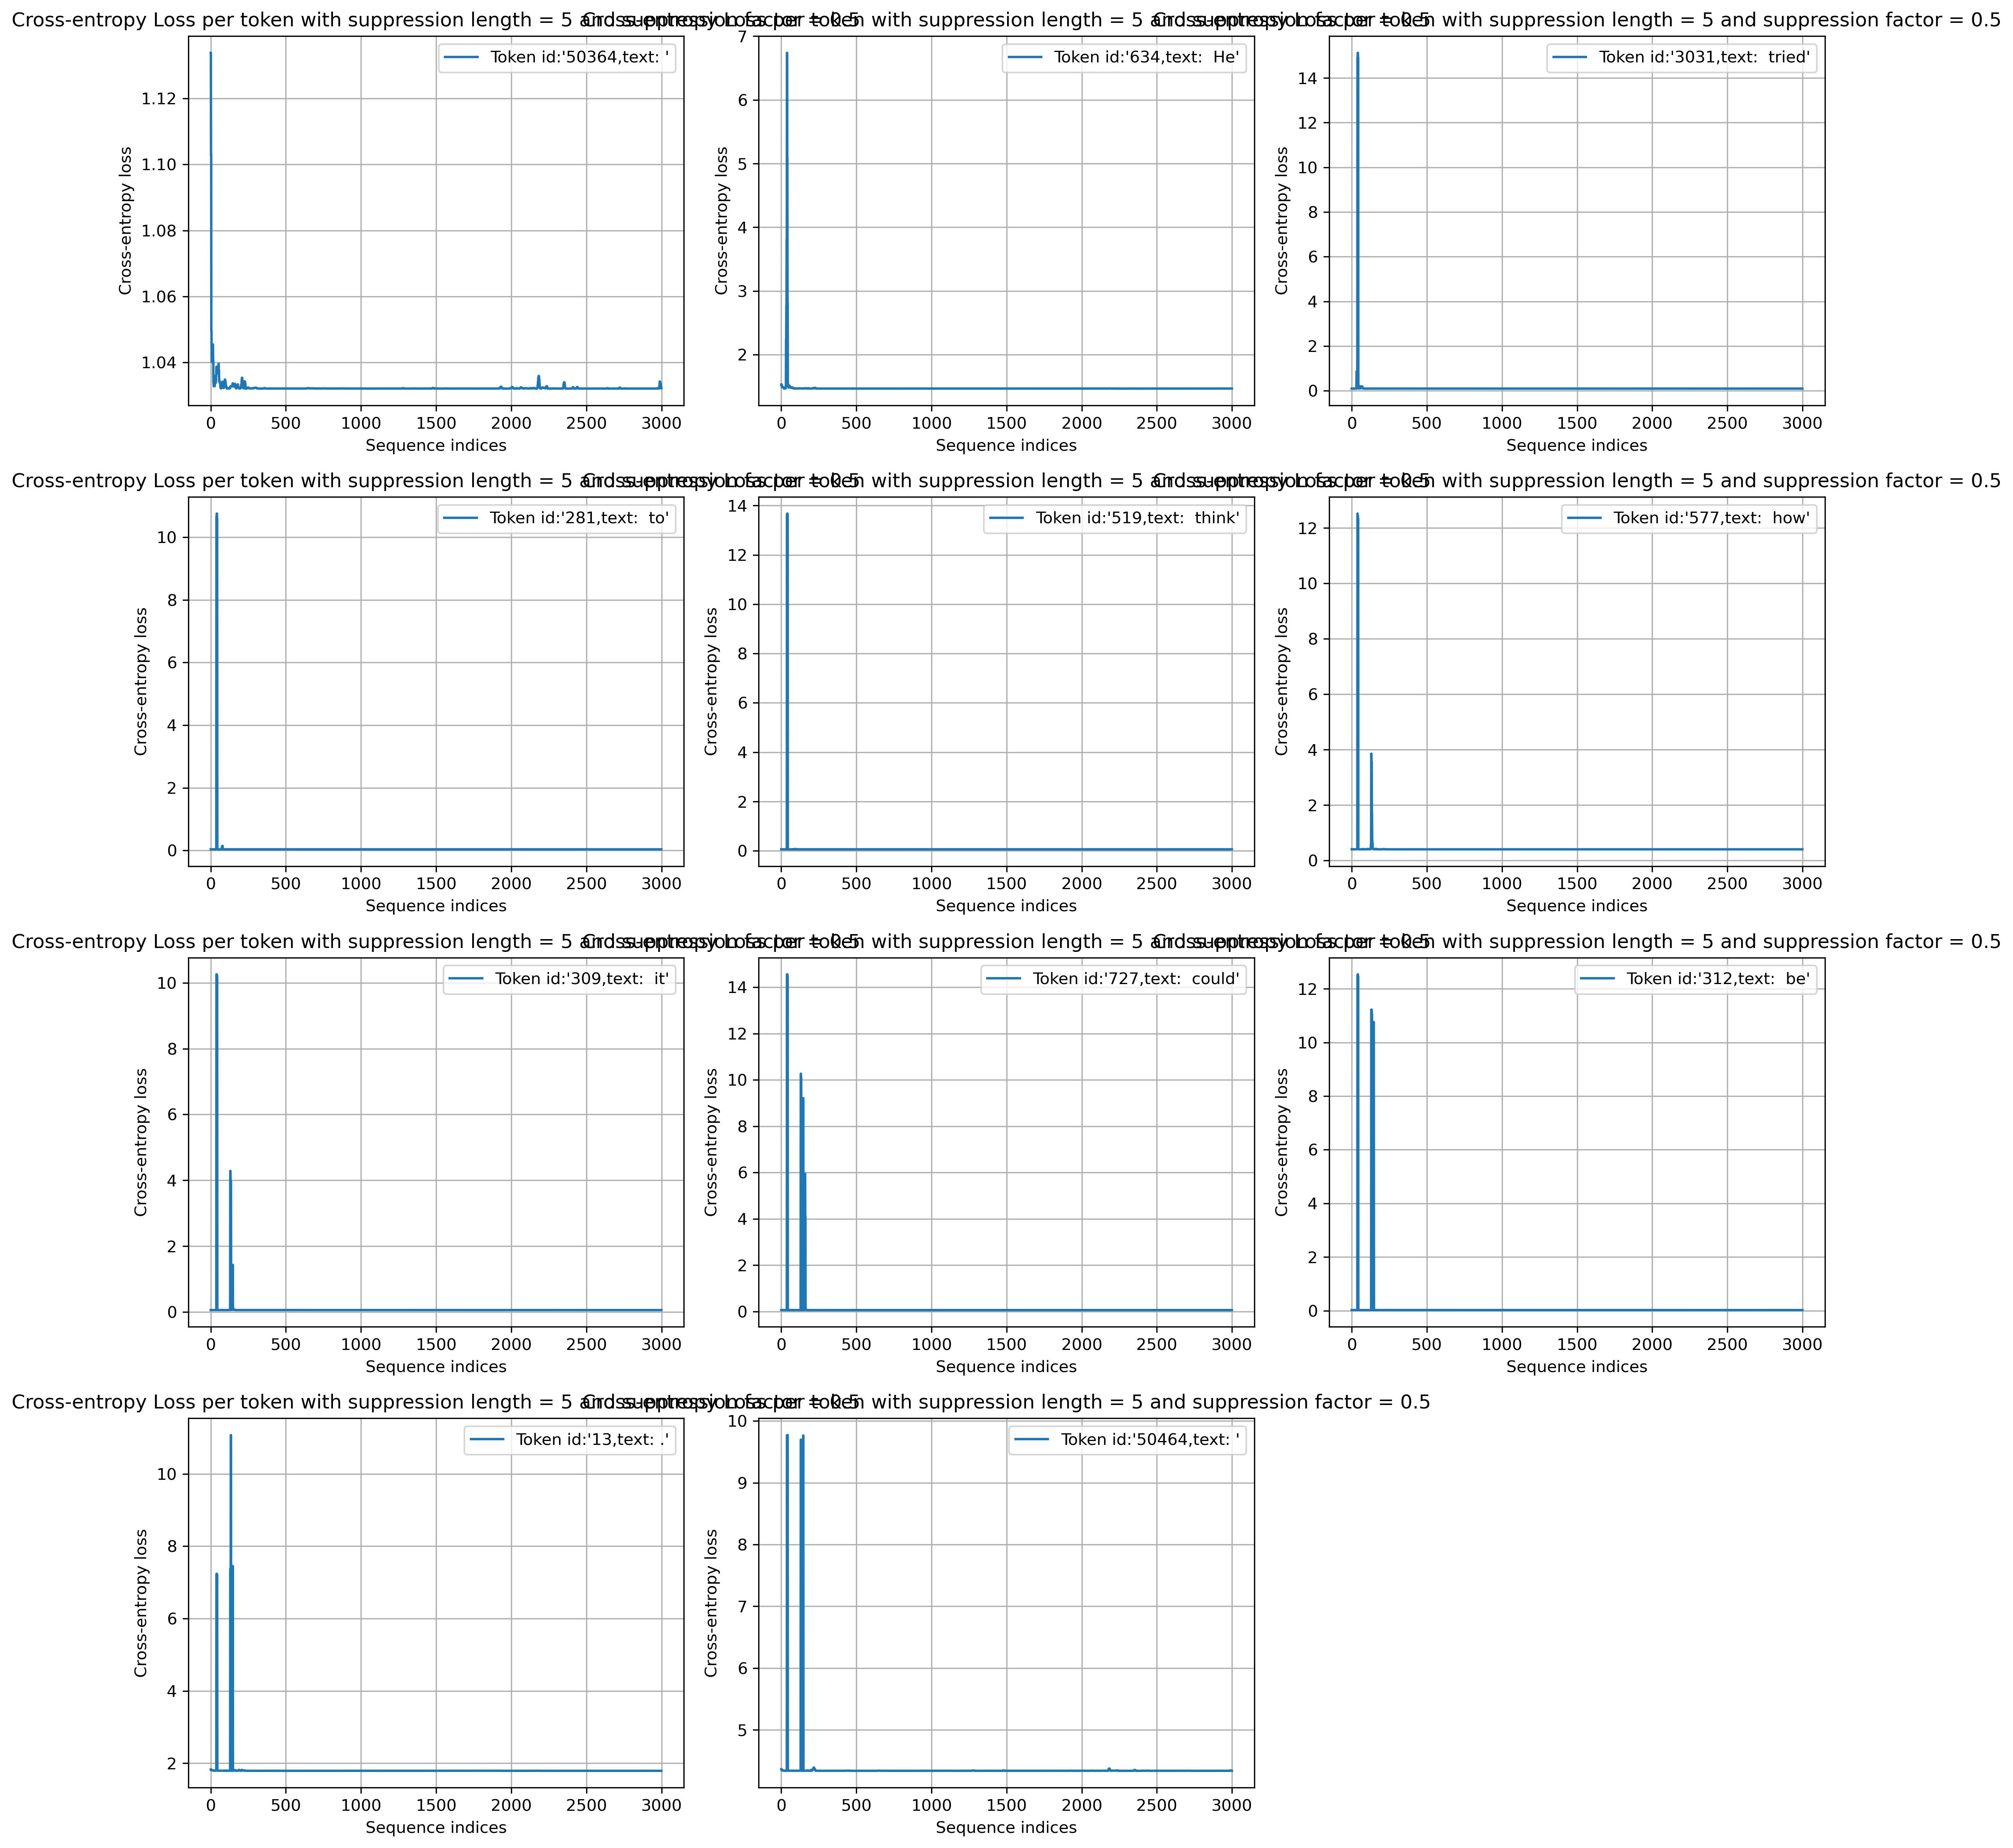
\includegraphics[width=\textwidth,height=0.5\textheight]{figures/loss_diff_sentence_5_word.png}
        \caption{Visualization set 5: (top) Log Mel spectrogram, (middle) sentence-level influence map, (bottom) token-level influence maps}
        \label{fig:viz_set5}
    \end{figure*}


    \end{document}

